\documentclass{standalone}
\usepackage{tikz,pgfplots}
\usepackage{newtxmath}

% definitions for interference images
\colorlet{wall}{blue!30!black}
\colorlet{myblue}{blue!70!black}
\colorlet{myorange}{orange!90!black!80}
\colorlet{myred}{red!70!black}
\colorlet{mydarkred}{red!50!black}
\colorlet{mylightgreen}{green!60!black!70}
\colorlet{mygreen}{green!60!black}
\colorlet{myredgrey}{red!50!black!80}
\colorlet{myshadow}{blue!30!black!90}
\tikzstyle{wave}=[myblue,thick]

\begin{document}

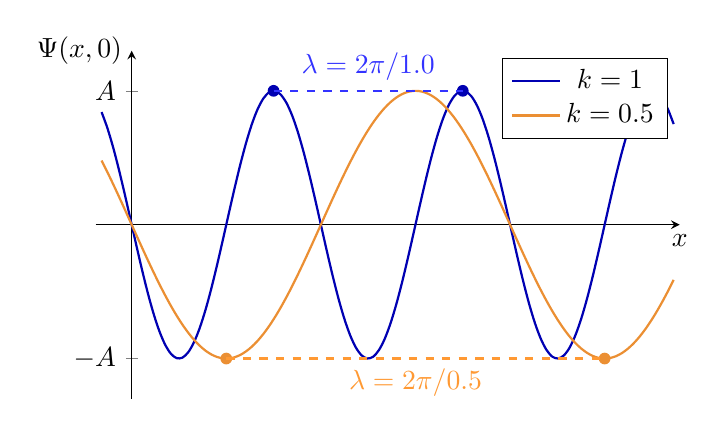
\begin{tikzpicture}
        \begin{axis}[xtick=\empty,
                    ytick={-1,1},
                    yticklabels={$-A$,$A$},
                    axis lines=middle,
                    enlarge x limits={abs=0.2},
                    enlarge y limits={abs=0.3},
                    x label style={anchor=north},
                    y label style={anchor=east},
                    xlabel={$x$},
                    ylabel={$\Psi(x,0)$},
                    width=9cm,
                    height=6cm]
        \addplot[domain=-1:18,samples=100,smooth,myblue,thick] {sin(deg(-x))};
        \addlegendentry{$k=1$}
        \addplot[domain=-1:18,samples=100,smooth,myorange,thick] {sin(deg(-0.5*x))};
        \addlegendentry{$k=0.5$}
        \node[circle,fill,inner sep=1.5pt,myblue] at (axis cs:3*pi/2,1) {};
        \node[circle,fill,inner sep=1.5pt,myblue] at (axis cs:7*pi/2,1) {};
        \draw[dashed, blue!80, thick] (axis cs:3*pi/2,1) -- node[above] {$\lambda=2\pi/1.0$} (axis cs:7*pi/2,1);
        \node[circle,fill,inner sep=1.5pt,myorange] at (axis cs:pi,-1) {};
        \node[circle,fill,inner sep=1.5pt,myorange] at (axis cs:5*pi,-1) {};
        \draw[dashed, orange!80, thick] (axis cs:pi,-1) -- node[below] {$\lambda=2\pi/0.5$} (axis cs:5*pi,-1);
        \end{axis}
\end{tikzpicture}

\end{document}